\documentclass[14pt]{extbook}
\usepackage{multicol, enumerate, enumitem, hyperref, color, soul, setspace, parskip, fancyhdr} %General Packages
\usepackage{amssymb, amsthm, amsmath, latexsym, units, mathtools} %Math Packages
\everymath{\displaystyle} %All math in Display Style
% Packages with additional options
\usepackage[headsep=0.5cm,headheight=12pt, left=1 in,right= 1 in,top= 1 in,bottom= 1 in]{geometry}
\usepackage[usenames,dvipsnames]{xcolor}
\usepackage{dashrule}  % Package to use the command below to create lines between items
\newcommand{\litem}[1]{\item#1\hspace*{-1cm}\rule{\textwidth}{0.4pt}}
\pagestyle{fancy}
\lhead{Progress Quiz 7}
\chead{}
\rhead{Version A}
\lfoot{3510-5252}
\cfoot{}
\rfoot{Summer C 2021}
\begin{document}

\begin{enumerate}
\litem{
Determine the domain of the function below.\[ f(x) = \frac{5}{36x^{2} -66 x + 30} \]\begin{enumerate}[label=\Alph*.]
\item \( \text{All Real numbers except } x = a, \text{ where } a \in [29.87, 30.11] \)
\item \( \text{All Real numbers.} \)
\item \( \text{All Real numbers except } x = a \text{ and } x = b, \text{ where } a \in [0.66, 0.99] \text{ and } b \in [0.96, 1.04] \)
\item \( \text{All Real numbers except } x = a \text{ and } x = b, \text{ where } a \in [29.87, 30.11] \text{ and } b \in [35.75, 36.14] \)
\item \( \text{All Real numbers except } x = a, \text{ where } a \in [0.66, 0.99] \)

\end{enumerate} }
\litem{
Choose the graph of the equation below.\[ f(x) = \frac{-1}{x - 1} + 2 \]\begin{enumerate}[label=\Alph*.]
\begin{multicols}{2}\item 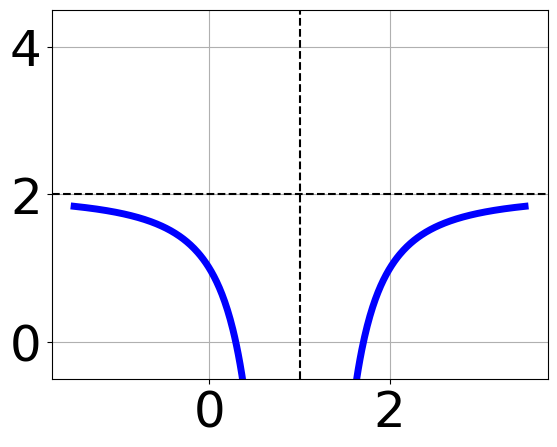
\includegraphics[width = 0.3\textwidth]{../Figures/rationalEquationToGraphAA.png}\item 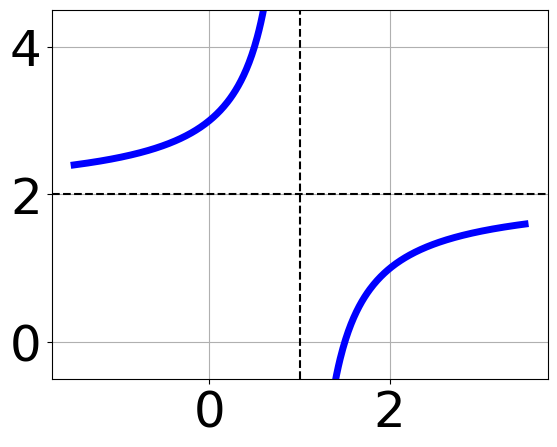
\includegraphics[width = 0.3\textwidth]{../Figures/rationalEquationToGraphBA.png}\item 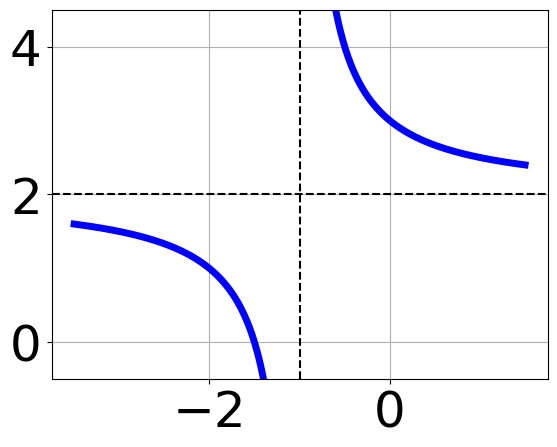
\includegraphics[width = 0.3\textwidth]{../Figures/rationalEquationToGraphCA.png}\item 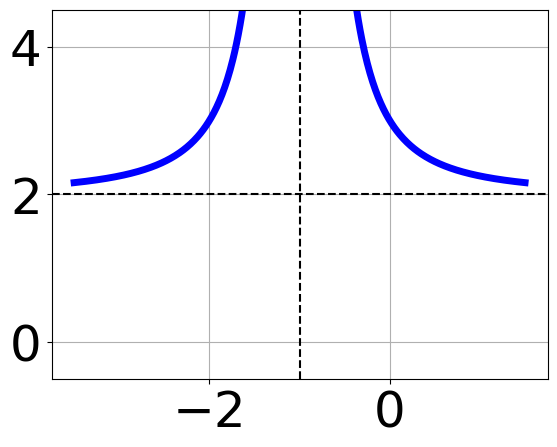
\includegraphics[width = 0.3\textwidth]{../Figures/rationalEquationToGraphDA.png}\end{multicols}\item None of the above.
\end{enumerate} }
\litem{
Choose the graph of the equation below.\[ f(x) = \frac{-1}{(x - 2)^2} + 1 \]\begin{enumerate}[label=\Alph*.]
\begin{multicols}{2}\item 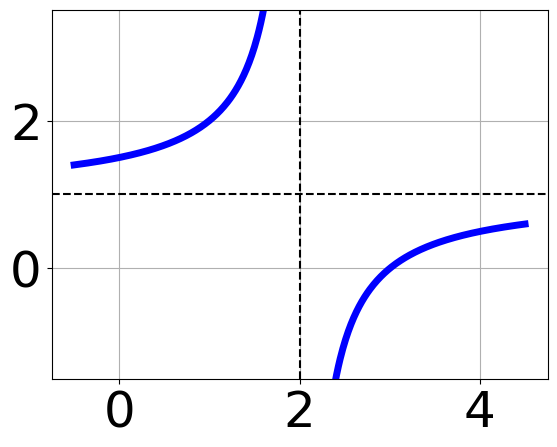
\includegraphics[width = 0.3\textwidth]{../Figures/rationalEquationToGraphCopyAA.png}\item 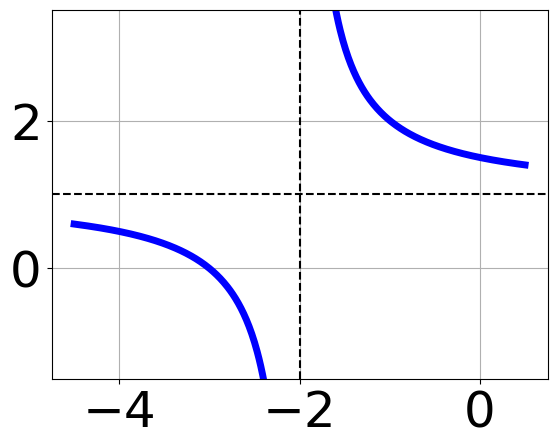
\includegraphics[width = 0.3\textwidth]{../Figures/rationalEquationToGraphCopyBA.png}\item 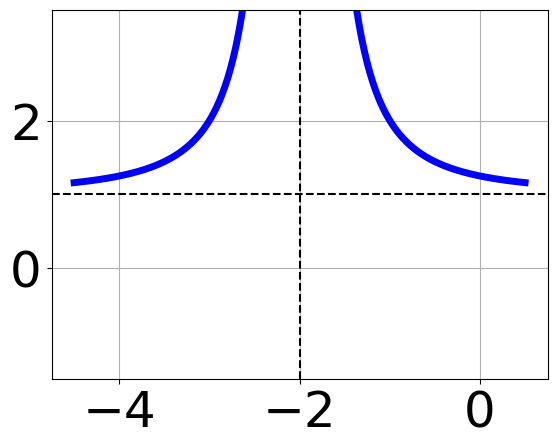
\includegraphics[width = 0.3\textwidth]{../Figures/rationalEquationToGraphCopyCA.png}\item 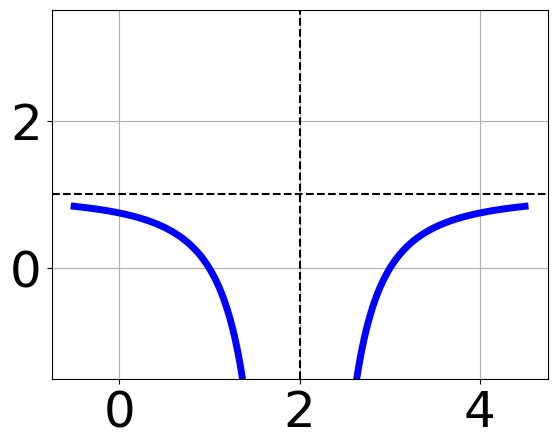
\includegraphics[width = 0.3\textwidth]{../Figures/rationalEquationToGraphCopyDA.png}\end{multicols}\item None of the above.
\end{enumerate} }
\litem{
Choose the equation of the function graphed below.
\begin{center}
    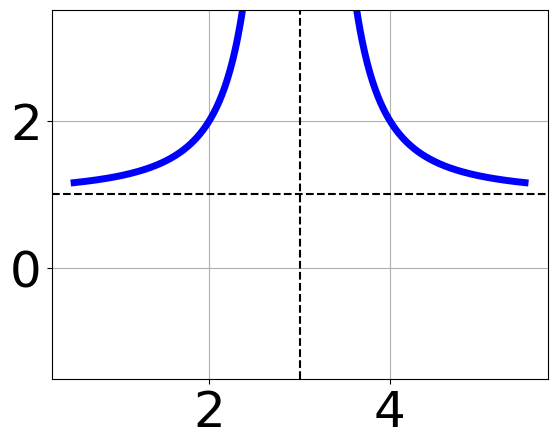
\includegraphics[width=0.5\textwidth]{../Figures/rationalGraphToEquationA.png}
\end{center}
\begin{enumerate}[label=\Alph*.]
\item \( f(x) = \frac{1}{(x + 3)^2} + 7 \)
\item \( f(x) = \frac{-1}{x - 3} + 7 \)
\item \( f(x) = \frac{-1}{(x - 3)^2} + 7 \)
\item \( f(x) = \frac{1}{x + 3} + 7 \)
\item \( \text{None of the above} \)

\end{enumerate} }
\litem{
Choose the equation of the function graphed below.
\begin{center}
    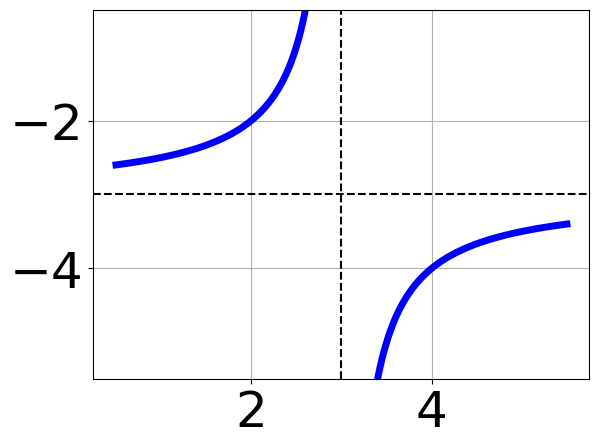
\includegraphics[width=0.5\textwidth]{../Figures/rationalGraphToEquationCopyA.png}
\end{center}
\begin{enumerate}[label=\Alph*.]
\item \( f(x) = \frac{-1}{(x - 3)^2} - 3 \)
\item \( f(x) = \frac{1}{(x + 3)^2} - 3 \)
\item \( f(x) = \frac{-1}{x - 3} - 3 \)
\item \( f(x) = \frac{1}{x + 3} - 3 \)
\item \( \text{None of the above} \)

\end{enumerate} }
\litem{
Solve the rational equation below. Then, choose the interval(s) that the solution(s) belongs to.\[ \frac{6}{-2x -3} + -5 = \frac{5}{-14x -21} \]\begin{enumerate}[label=\Alph*.]
\item \( x \in [-1.03,1.97] \)
\item \( \text{All solutions lead to invalid or complex values in the equation.} \)
\item \( x_1 \in [-2.03, 0.97] \text{ and } x_2 \in [-0.03,1.97] \)
\item \( x \in [-2.03,-0.03] \)
\item \( x_1 \in [-2.03, 0.97] \text{ and } x_2 \in [-1.6,0.4] \)

\end{enumerate} }
\litem{
Solve the rational equation below. Then, choose the interval(s) that the solution(s) belongs to.\[ \frac{-2}{-8x + 2} + -2 = \frac{-9}{24x -6} \]\begin{enumerate}[label=\Alph*.]
\item \( x \in [-2.44,1.56] \)
\item \( x_1 \in [-0.04, 0.14] \text{ and } x_2 \in [0.56,3.56] \)
\item \( x \in [-0.04,0.14] \)
\item \( \text{All solutions lead to invalid or complex values in the equation.} \)
\item \( x_1 \in [-0.22, -0] \text{ and } x_2 \in [0.56,3.56] \)

\end{enumerate} }
\litem{
Determine the domain of the function below.\[ f(x) = \frac{4}{12x^{2} +39 x + 30} \]\begin{enumerate}[label=\Alph*.]
\item \( \text{All Real numbers except } x = a \text{ and } x = b, \text{ where } a \in [-20.06, -19.04] \text{ and } b \in [-18.48, -16.42] \)
\item \( \text{All Real numbers except } x = a, \text{ where } a \in [-2.49, -1.52] \)
\item \( \text{All Real numbers except } x = a, \text{ where } a \in [-20.06, -19.04] \)
\item \( \text{All Real numbers except } x = a \text{ and } x = b, \text{ where } a \in [-2.49, -1.52] \text{ and } b \in [-1.37, -1.17] \)
\item \( \text{All Real numbers.} \)

\end{enumerate} }
\litem{
Solve the rational equation below. Then, choose the interval(s) that the solution(s) belongs to.\[ \frac{7x}{4x -3} + \frac{-7x^{2}}{-20x^{2} +39 x -18} = \frac{3}{-5x + 6} \]\begin{enumerate}[label=\Alph*.]
\item \( x \in [1.08,1.38] \)
\item \( \text{All solutions lead to invalid or complex values in the equation.} \)
\item \( x_1 \in [-0.3, 0.02] \text{ and } x_2 \in [0.37,0.85] \)
\item \( x_1 \in [-0.3, 0.02] \text{ and } x_2 \in [0.81,1.28] \)
\item \( x \in [0.92,1.12] \)

\end{enumerate} }
\litem{
Solve the rational equation below. Then, choose the interval(s) that the solution(s) belongs to.\[ \frac{2x}{4x + 6} + \frac{-6x^{2}}{24x^{2} +56 x + 30} = \frac{-6}{6x + 5} \]\begin{enumerate}[label=\Alph*.]
\item \( x \in [-1.37,1.64] \)
\item \( \text{All solutions lead to invalid or complex values in the equation.} \)
\item \( x \in [-2.74,-1.09] \)
\item \( x_1 \in [-4.68, -3.43] \text{ and } x_2 \in [-1.48,-1.33] \)
\item \( x_1 \in [-4.68, -3.43] \text{ and } x_2 \in [-1.54,-1.46] \)

\end{enumerate} }
\end{enumerate}

\end{document}